% Stokes: dos superficies adyacentes; los bordes internos se cancelan (libro fig. 2.13)
\documentclass[border=5pt]{standalone}
\usepackage{tikz}
\usetikzlibrary{arrows.meta, calc}
\begin{document}
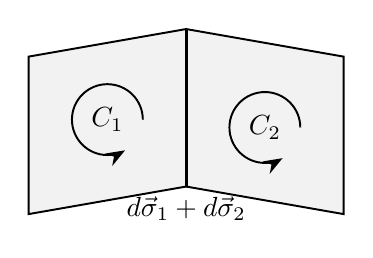
\begin{tikzpicture}[>={Stealth[length=2.4mm]}, line width=0.7pt]
  % dos parches que comparten el borde central
  \fill[black!5] (0,0)--(2,0.35)--(2,2.35)--(0,2.0)--cycle;
  \fill[black!5] (2,0.35)--(4,0)--(4,2.0)--(2,2.35)--cycle;
  \draw (0,0)--(2,0.35)--(2,2.35)--(0,2.0)--cycle;
  \draw (2,0.35)--(4,0)--(4,2.0)--(2,2.35);
  % borde común
  \draw[line width=1pt] (2,0.35)--(2,2.35);
  % circulaciones
  \draw[->] (1.0,1.2)+(0.45,0) arc (0:300:0.45); \node at (1.0,1.2){$C_1$};
  \draw[->] (3.0,1.1)+(0.45,0) arc (0:300:0.45); \node at (3.0,1.1){$C_2$};
  \node[below] at (2,0.35){$d\vec\sigma_1+d\vec\sigma_2$};
\end{tikzpicture}
\end{document}
